There are several types of low-level task the surgeon usually employs while
performing the surgery.

One common procedure is reconnection and joining of blood vessels. Another
is fixing the stenosis of aorta where the three most common types of fixing
the problem are:

\begin{description}

  \item[End to end aortoplasty:] the surgeon completely cuts away the
    affected part of aorta and sutures the two ends of aorta back together.

  \item[Patch aortoplasty:] the surgeon performs a cut along the axis of
    the aorta thus allowing the narrow place to expand. Then applies a
    patch from artificial material to fill the hole in.

  \item[Subclavian flap aortoplasty:] the nearest artery is cut,
    removing also half of the artery (along the axis) and part of the
    aorta in the affected place. He then uses the rest of the artery to
    patch the aorta.

\end{description}

From our point of view the all these procedures share the same similarity:
parts of the circulatory system are sutured together or to a patch. These
parts are not too far away from each other. On this we have based our
general approach in the simulation. The simple way how to perform the
suturing would be to connect the respective edges with springs. This
approach however adds some unwanted energy to the system. Our method is
based solely on the relaxation of the mesh of shell elements.

We start with a mesh representing the situation after all the cuts have
been performed but before suturing takes place. In the first step we select
on the mesh edges that we want to suture together and join the
corresponding nodes together. The result is topologicaly different mesh
that has same number of elements. The Figure. \ref{fig-JoiningVessels} explains
this operation. Then we start the simulation on the modified mesh while
using the original mesh to define rest shapes of the shell elements. After
the mesh relaxes and the simulation reaches energetical equilibrium the
simulation terminates.

\begin{figure}[tbh]
\begin{center}
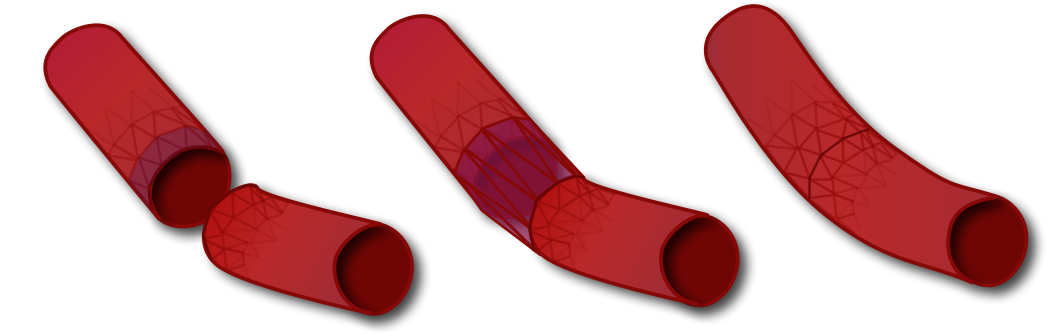
\includegraphics[width=\columnwidth]{img/rest_shape_scheme.png}
\end{center}

\caption{Scheme showing the method for joining two vessels.}
\label{fig-JoiningVessels}
\end{figure}

If the nodes that are to be sutured together are not in a close vicinity we
may experience unwanted quick increase of internal forces at the beginning
of the simulation. To allevieate this problem we have implemented the
techinuqe of linear interpolation of the rest shape mesh. At the start of
the simulation we use different rest shape mesh. It is topologicaly
equivalent to the original mesh but nodes have positions equivalent to the
simulated mesh (that way the initial deformations are not so big). During
the simulation we then perform several steps of linear interpolation
between these two rest shape meshes. At the end of interpolation the
original rest shape is used. After the mesh relaxes the simulation again
terminates.

% vim: et sw=2 tw=75 fdm=marker fdc=2 spell
